\documentclass[a4paper,9pt]{extarticle}

\usepackage[margin=10.5mm,top=9mm,bottom=9mm]{geometry}
% LuaLaTeX + TeX Live 標準の日本語フォントを使用。
% fontspec や \setmainfont などのシステムフォント指定は不要。
\usepackage{luatexja}

\usepackage{amsmath,amssymb,mathtools}
\usepackage[dvipsnames]{xcolor}
\usepackage[most]{tcolorbox}
\usepackage{multicol}
\usepackage{tikz}
\usetikzlibrary{calc}
\usepackage{enumitem}
\usepackage{microtype}

\setlength{\parindent}{0pt}
\setlength{\parskip}{1.2pt}
\setlength{\columnsep}{7mm}
\setlength{\columnseprule}{0.25pt}
\setlength{\abovedisplayskip}{2.3pt}
\setlength{\belowdisplayskip}{2.3pt}
\setlength{\abovedisplayshortskip}{1.5pt}
\setlength{\belowdisplayshortskip}{1.5pt}
\linespread{0.98}
\pagestyle{empty}

\definecolor{mainblue}{RGB}{38,72,108}
\definecolor{paleblue}{RGB}{241,246,251}
\definecolor{palegray}{RGB}{247,247,247}

\newtcolorbox{problembox}{
  enhanced,
  colback=paleblue,colframe=mainblue,
  boxrule=0.75pt,arc=1.2mm,
  left=2.7mm,right=2.7mm,top=1.4mm,bottom=1.4mm,
  title={\sffamily\bfseries 問題},
  coltitle=white,colbacktitle=mainblue,
  fonttitle=\normalsize
}

\newtcolorbox{keybox}{
  enhanced,
  colback=palegray,colframe=black!55,
  boxrule=0.55pt,arc=1mm,
  left=2mm,right=2mm,top=1.2mm,bottom=1.2mm
}

\newtcolorbox{answerbox}{
  enhanced,
  colback=white,colframe=mainblue,
  boxrule=1pt,arc=1.2mm,
  left=3mm,right=3mm,top=1.5mm,bottom=1.5mm,
  title={\sffamily\bfseries 結論},
  coltitle=white,colbacktitle=mainblue,
  fonttitle=\normalsize
}

\newcommand{\vect}[1]{\overrightarrow{#1}}
\newcommand{\stephead}[1]{\vspace{1.5pt}{\sffamily\bfseries #1}\par}

\begin{document}

\begin{problembox}
複素数平面上で，3点 $O(0),\ A(\alpha),\ B(\beta)$ は三角形の3頂点であり，
\[
  \alpha^7+\beta^7=(\alpha+\beta)^7
\]
をみたすとする。このとき $\triangle OAB$ はどのような三角形か。
\end{problembox}

\begin{multicols}{2}

\[
 \gamma=\alpha+\beta,\qquad \delta=\alpha-\beta
\]
とおくと，
\[
 \alpha=\frac{\gamma+\delta}{2},\qquad
 \beta=\frac{\gamma-\delta}{2}.
\]
条件式へ代入して
\[
 \left(\frac{\gamma+\delta}{2}\right)^7+
 \left(\frac{\gamma-\delta}{2}\right)^7=\gamma^7,
\]
したがって
\[
 (\gamma+\delta)^7+(\gamma-\delta)^7=128\gamma^7.
\]
左辺で$\delta$ の奇数次の項は消えるので
\[
\begin{aligned}
 2\gamma^7+42\gamma^5\delta^2
 &+70\gamma^3\delta^4\\
 &+14\gamma\delta^6=128\gamma^7.
\end{aligned}
\]

三角形になるので$\gamma\neq0$であるので、$\div14\gamma$して
\[
\begin{aligned}
\delta^6+5\gamma^2\delta^4+3\gamma^4\delta^2-9\gamma^6=0.
\end{aligned}
\]
これは$\delta^2$の3次式なので、
\[
 \boxed{(\delta^2-\gamma^2)(\delta^2+3\gamma^2)^2=0}.
\]

\stephead{2．退化する解を除く}
$\delta^2=\gamma^2$ なら $\delta=\pm\gamma$。これは
\[
 \alpha-\beta=\pm(\alpha+\beta)
\]
を意味し，$\alpha=0$ または $\beta=0$ となるため，三角形をつくらない。したがって
\[
 \delta^2=-3\gamma^2,
 \qquad
 \boxed{\delta=\pm i\sqrt3\,\gamma}.
\]

\columnbreak


$M$ を辺 $AB$ の中点とする。このとき
\[
 M=\frac{\alpha+\beta}{2}=\frac{\gamma}{2},
 \qquad
 \vect{BA}=\alpha-\beta=\delta.
\]
したがって
\[
 OM\parallel\gamma,
 \qquad AB\parallel\delta,
\]
であるから $OM\perp AB$。しかも $M$ は $AB$ の中点なので，$O$ は $AB$ の垂直二等分線上にある。よって
\[
 OA=OB.
\]
さらに，
\[
\begin{aligned}
 AB&=|\delta|=\sqrt3|\gamma|,\\
 OM&=\frac{|\gamma|}{2},\qquad
 AM=\frac{\sqrt3|\gamma|}{2}.
\end{aligned}
\]
直角三角形 $OAM$ に三平方の定理を用いると，
\[
\begin{aligned}
 OA^2&=OM^2+AM^2\\
 &=\left(\frac{|\gamma|}{2}\right)^2
  +\left(\frac{\sqrt3|\gamma|}{2}\right)^2\\
 &=|\gamma|^2.
\end{aligned}
\]
したがって
\[
 OA=OB=|\gamma|,
 \qquad AB=\sqrt3|\gamma|,
\]
すなわち
\[
 \boxed{OA:OB:AB=1:1:\sqrt3}.
\]
辺の比 $1:1:\sqrt3$ より，$AB$ の対角は $120^\circ$，残りの2角はそれぞれ $30^\circ$ である。

\end{multicols}

\vspace{-2mm}
\begin{answerbox}
\begin{minipage}[c]{0.73\linewidth}
$\triangle OAB$ は二等辺三角形であり，
\[
 \angle AOB=120^\circ,
 \qquad \angle OAB=\angle OBA=30^\circ.
\]
したがって，\textbf{頂角 $120^\circ$ の二等辺三角形}である。
\end{minipage}
\hfill
\begin{minipage}[c]{0.23\linewidth}
\centering
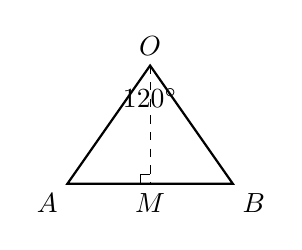
\begin{tikzpicture}[scale=0.60]
 \coordinate (O) at (0,2.5);
 \coordinate (A) at (-1.75,0);
 \coordinate (B) at (1.75,0);
 \coordinate (M) at (0,0);
 \draw[thick] (O)--(A)--(B)--cycle;
 \draw[dashed] (O)--(M);
 \draw ($(M)+(-0.20,0)$)--($(M)+(-0.20,0.20)$)--($(M)+(0,0.20)$);
 \node[above] at (O) {$O$};
 \node[below left] at (A) {$A$};
 \node[below right] at (B) {$B$};
 \node[below] at (M) {$M$};
 \node at (0,1.82) {$120^\circ$};
\end{tikzpicture}
\end{minipage}
\end{answerbox}

\end{document}
